%!TEX root = ../main.tex
\chapter{Validation} % (fold)
\label{cha:validation}

\section{Presentation of the toy problems}

To demonstrate the capacities and the limitations of
the harmonic balance approach, two toy problems are set up.
The first one solves the constant convection equation within 
a harmonic balance framework, the second one is a laminar
Navier-Stokes rotating blocks configuration.

\subsection{Convection equation problem} % (fold)
\label{sub:convection_equation_problem}

The harmonic balance source term is an alternative to
a classical time marching scheme for periodic phenomenon.
The simplest unsteady equation
that can be formulated is the constant convection equation:
\begin{equation}
  \label{eq:convection}
  \frac{\partial u}{\partial t} + c \frac{\partial u}{\partial x} = 0,
\end{equation}
where $c$ denotes the constant velocity and $u$ the transported quantity.
If we impose an unsteady periodic inlet,
we obtain a simple test case for harmonic balance approach. Any kind
of input can be simulated allowing to fully investigate the properties of 
the method.

Moreover, this equation is interesting as the analytical solution is simple
and known for any input. In fact, the solution only depends on the 
initial and/or boundary conditions:
\begin{equation}
  \label{eq:solconvanalytic}
    u(x, t) = u_0(x - ct)
\end{equation}
where $u_0$ is the boundary condition. Moreover, as the equation
is simple enough, it will be easy to discriminate the effects of the
harmonic balance source term.

The convection equation is solved in a 1D cartesian mesh.
A $4$\textsuperscript{th} order centered finite
difference scheme is used to evaluate the spatial derivative:
\begin{equation}
    \left. \frac{\partial u}{\partial x} \right)_{t=q}^{x=i} \approx 
    \frac{-u^{i+2}_{q} + 8 u^{i+1}_{q} - 8 u^{i-1}_{q} + u^{i-2}_{q}}{12\Delta x},
    \label{eq:convection_center4}
\end{equation}
where $u_i^q$ is the sum of the velocity for  
all harmonic balance instants as defined in Eq.~\eqref{eq:hb_concatenation},
evaluated at position $i$ within pseudo-iteration $q$.
A $4$ step Runge-Kutta method is then use to time 
march the equation to the steady state with the coefficients $\alpha_0 = 0$,
$\alpha_1 = 1/4$, $\alpha_2 = 1/3$, $\alpha_3 = 1/2$ and $\alpha_4 = 1$.
The k\textsuperscript{th} step is evaluated by:
\begin{equation}
    u_k = u_q - \alpha_k \Delta t \left [ 
          c \left. \frac{\partial u_{k-1}}{\partial x} \right)_{t=t_q + \alpha_{k-1} \Delta t}
          + D_t(u_q)
          \right],
    \label{eq:convection_rk4}
\end{equation}
where the HB source term $D_t(u_q)$ is computed using Eq.~\eqref{eq:dt}. 

As we use 
an explicit time marching scheme, the CFL number is set to $1$ to ensure stability.
The mesh is composed of $2000$ grid points, which proved to be converged.
The period of injection is chosen so that, when the temporal frequency is
set to $1$, only one pattern 
appears at a time in the mesh
as shown in Fig.~\ref{fig:convection_injection_paper} for a Gaussian function.
This is done by setting the biggest temporal period $T$ to:
\begin{equation}
   T = \frac{L_x}{c},
\end{equation}
where $L_x$ is the size of the mesh.


As the harmonic balance computations are steady computations linked 
by a source term, 
different boundary conditions, as done in~\cite{Dufour2010},
have to be set to impose a periodic injection. Two ghost cells
are used to maintain the spatial $4$\textsuperscript{th} order scheme 
at the left
boundary condition.
\begin{figure}[htbp]
  \begin{center}
    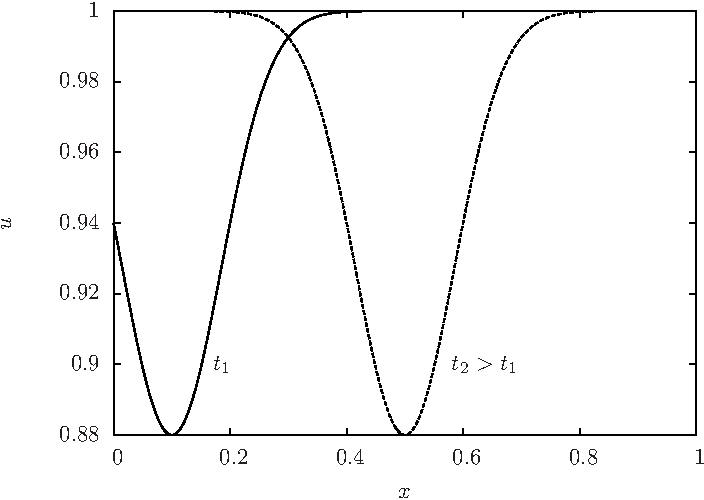
\includegraphics[width=.5\textwidth]{GAUSSIAN_INJECTION_PAPER.pdf}
  \end{center}
  \caption{Convection of the Gaussian function in the 1D cartesian mesh.}
  \label{fig:convection_injection_paper}
\end{figure}
For the right boundary condition, imposing a periodicity condition is
numerically stiff. For this reason, the scheme is degenerated 
to an upwind scheme to avoid wave reflections. The upwind scheme is degenerated to
a 2\textsuperscript{nd} order, one cell before and at first order on the 
last cell:
\begin{align}
    \left. \frac{\partial u}{\partial x} \right)_{t=q}^{x=m-1} &\approx 
    \frac{3 u^{m-1}_{q} - 4 u^{m-2}_{q} + u^{m-3}_{q}}{2\Delta x}, \\
    \left. \frac{\partial u}{\partial x} \right)_{t=q}^{x=m} &\approx 
    \frac{u^{m}_{q} - u^{m-1}_{q}}{\Delta x},
\label{eq:upwind_scheme}
\end{align}
where $m$ is the total number of grid points. This is much better than a periodicity
condition as the convected function suffers from diffusion and dispersion (even if the
mesh is small enough) that is not compatible with the injected function.

% chapter validation (end)